\documentclass[tikz,border=10pt]{standalone}
\usepackage[utf8]{inputenc}
\usepackage{amsmath, amssymb}
\usetikzlibrary{arrows.meta, positioning, calc, shapes.geometric}

\begin{document}

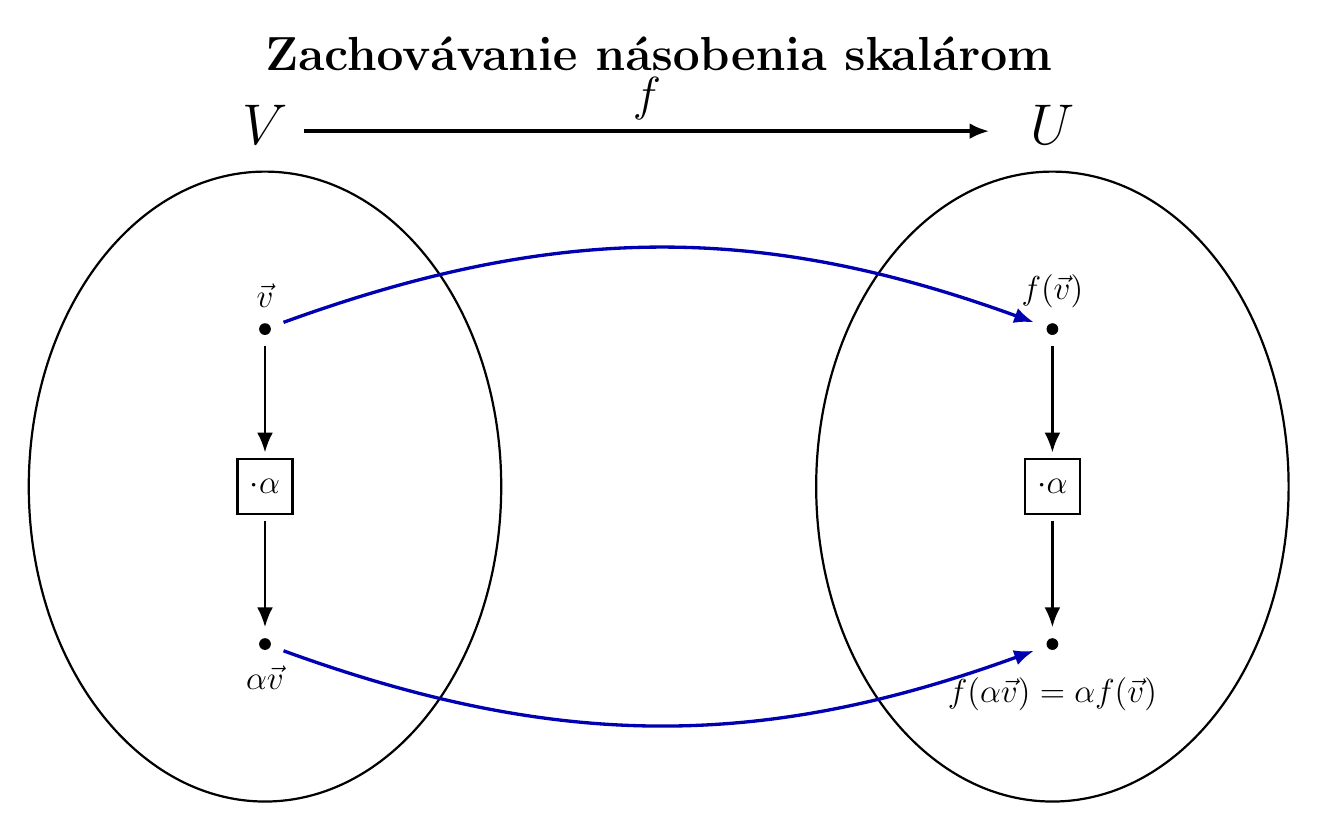
\begin{tikzpicture}[
    thick,
    >={Latex[length=2.5mm, width=2mm]}, % Define nice arrowheads
    dot/.style={circle, fill=black, inner sep=1.5pt, outer sep=2pt}, % Style for vector points
    % Adapted from addbox in the provided snippet for scalar multiplication
    multbox/.style={draw, rectangle, minimum size=0.7cm, font=\large}, 
    set ellipse/.style={draw, ellipse, minimum width=6cm, minimum height=8cm}, % Style for the sets V and U
    map arrow/.style={->, shorten >=3pt, shorten <=3pt, very thick, color=blue!70!black}, % Style for mapping arrows
    internal arrow/.style={->, shorten >=2pt, shorten <=2pt} % Style for arrows inside the sets
]

    % === Title ===
    \node[font=\LARGE\bfseries, align=center] at (5, 5.5) {Zachovávanie násobenia skalárom};

    % === Coordinates for Set Centers ===
    \coordinate (V_center) at (0,0);
    \coordinate (U_center) at (10,0);

    % === Draw Sets V and U ===
    \node[set ellipse] (SetV) at (V_center) {};
    \node[set ellipse] (SetU) at (U_center) {};

    % Labels for sets
    \node[above=0.2cm of SetV, font=\huge] {$V$};
    \node[above=0.2cm of SetU, font=\huge] {$U$};

    % Top mapping arrow f
    \draw[->, line width=1.5pt] ($(SetV.north)+(0.5,0.5)$) -- node[above, font=\LARGE] {$f$} ($(SetU.north)+(-0.8,0.5)$);


    % ====== INSIDE SET V ======
    % Define positions
    \coordinate (v_pos) at (0, 2);
    \coordinate (box_V_pos) at (0, 0);
    \coordinate (av_pos) at (0, -2);

    % Draw elements
    \node[dot, label={[font=\large]above:$\vec{v}$}] (v_node) at (v_pos) {};
    \node[multbox] (mult_V) at (box_V_pos) {$\cdot \alpha$};
    \node[dot, label={[font=\large]below:$\alpha\vec{v}$}] (av_node) at (av_pos) {};

    % Draw internal arrows showing scalar multiplication
    \draw[internal arrow] (v_node) -- (mult_V);
    \draw[internal arrow] (mult_V) -- (av_node);


    % ====== INSIDE SET U ======
    % Define relative positions (shifted by U_center)
    \coordinate (fv_pos) at ($(U_center)+(0, 2)$);
    \coordinate (box_U_pos) at ($(U_center)+(0, 0)$);
    \coordinate (afv_pos) at ($(U_center)+(0, -2)$);

    % Draw elements
    \node[dot, label={[font=\large]above:$f(\vec{v})$}] (fv_node) at (fv_pos) {};
    \node[multbox] (mult_U) at (box_U_pos) {$\cdot \alpha$};
    \node[dot] (result_node) at (afv_pos) {};

    % Label for the result showing the preservation property
    \node[below=0.3cm, align=center, font=\large] at (result_node) {$f(\alpha\vec{v}) = \alpha f(\vec{v})$};

    % Draw internal arrows showing scalar multiplication in U
    \draw[internal arrow] (fv_node) -- (mult_U);
    \draw[internal arrow] (mult_U) -- (result_node);


    % ====== MAPPING ARROWS BETWEEN V AND U ======
    % Map the vector
    \draw[map arrow] (v_node) to[bend left=20] (fv_node);

    % Map the scaled vector
    \draw[map arrow] (av_node) to[bend right=20] (result_node);

\end{tikzpicture}
\end{document}
